\chapter{Compare Ray Results with Other Distributed Computing Tools}

\vspace{0.3cm}
As outlined in the preceding chapter, the implementation of a scalable architectures for AI models utilizing Ray, a robust distributed computing framework, facilitates seamless autoscaling and the efficient distribution of computational resources within a cloud-native architectures \cite{moritz}. This chapter examined the ways in which the fundamental modules of Ray comprising Ray Data, Ray Tune, Ray Train, Ray Serve and RLlib facilitate distributed data processing, hyperparameter optimization, model training and serving tasks within a unified ecosystem. The objective of this chapter is to present a comprehensive comparison between the Ray ecosystem and other prominent tools in the distributed computing domain, including Apache Spark, Dask, Modin, Optuna, Hyperopt and TensorFlow Serve. This comparison is intended to highlight the different features and capabilities of Ray and to assist users in selecting the most appropriate framework based on their specific use cases whether they are focused on machine learning, data processing or large-scale computations \cite{ray_doc}.

\section{Distributed Computing Tools}


This section provides an overview of popular distributed computing frameworks, including Apache Spark, Hadoop, Modin, Dask, Optuna, Hyperopt and TensorFlow. These technologies are essential in supporting big data and are used to facilitate scalable data processing over distributed environments. They form the core of the distributed computing technology stack, allowing organisations to manage, process and analyse large volumes of data across clusters seamlessly and are therefore essential tools in modern big data applications.
 \cite{sun2023survey}


\subsection{Hadoop}
Apache Hadoop is an open source technology that creates an infrastructure for managing big data across multiple nodes or resources which makes it suitable for big data applications. The
Hadoop ecosystem is made of combining of different software packages it offers different functionality for different scenarios. For example Hadoop distributed file system \abk{HDFS}{Hadoop Distributed File System} manages process to store files in distributed manner, whereas Hadoop MapReduce is a software framework which helps to execute MapReduce algorithm for larger distributed datasets in clusters. These software components work together seamlessly in clusters or cloud-native environments to perform tasks for a variety of applications. Hadoop uses a master slave architecture to efficiently store and process large amounts of data. During task execution, the master node distributes sub tasks to the slave nodes, which store local blocks of data and perform computations on that data locally. \cite{ketu2020performance, sun2023survey}

\textbf{Hadoop Distributed File System}

HDFS is the block storage layer that Hadoop uses to manage its files, designed to handle very large datasets with high reliability. HDFS uses data replication to ensure data integrity and availability, this replication allows HDFS to efficiently stream large amounts of data to applications in a timely manner. Its architecture consists of two main components, the NameNode and the DataNodes, which operate in a master slave setup. The NameNode manages the metadata that tracks where files are stored in the system, while the DataNodes handle the actual data storage. HDFS operates as a single writer, multiple reader file system, meaning that once a client opens a file for writing, it has exclusive access until the operation is complete. Once a file is closed, its contents cannot be modified or removed, although additional data can be appended by reopening the file. Over time, HDFS has undergone numerous improvements that have increased its flexibility and enabled it to support different approaches to MapReduce computation. \cite{polato2014comprehensive}

\textbf{MapReduce}

A job in Hadoop consists primarily of two key functions, the map function and the reduce function. In addition, there are other functions that can be executed after the map function or between the map and reduce functions. The main role of the map function is to read chunks of data from HDFS and convert them into key/value pairs with different partitions. For example, in text mining, the map function acts as a parser and cleaner for the dataset, as shown \autoref{fig:MapReduce}, where the input data is divided among multiple mappers, followed by the reduce tasks to perform parallel computations. Also shown in \autoref{fig:MapReduce}, the output from the mapping stage is fed into various reducers. These reducers then process the input key/value pairs to perform operations such as summing or averaging the values. \cite{ketu2020performance}

\begin{figure}[h]
\centering
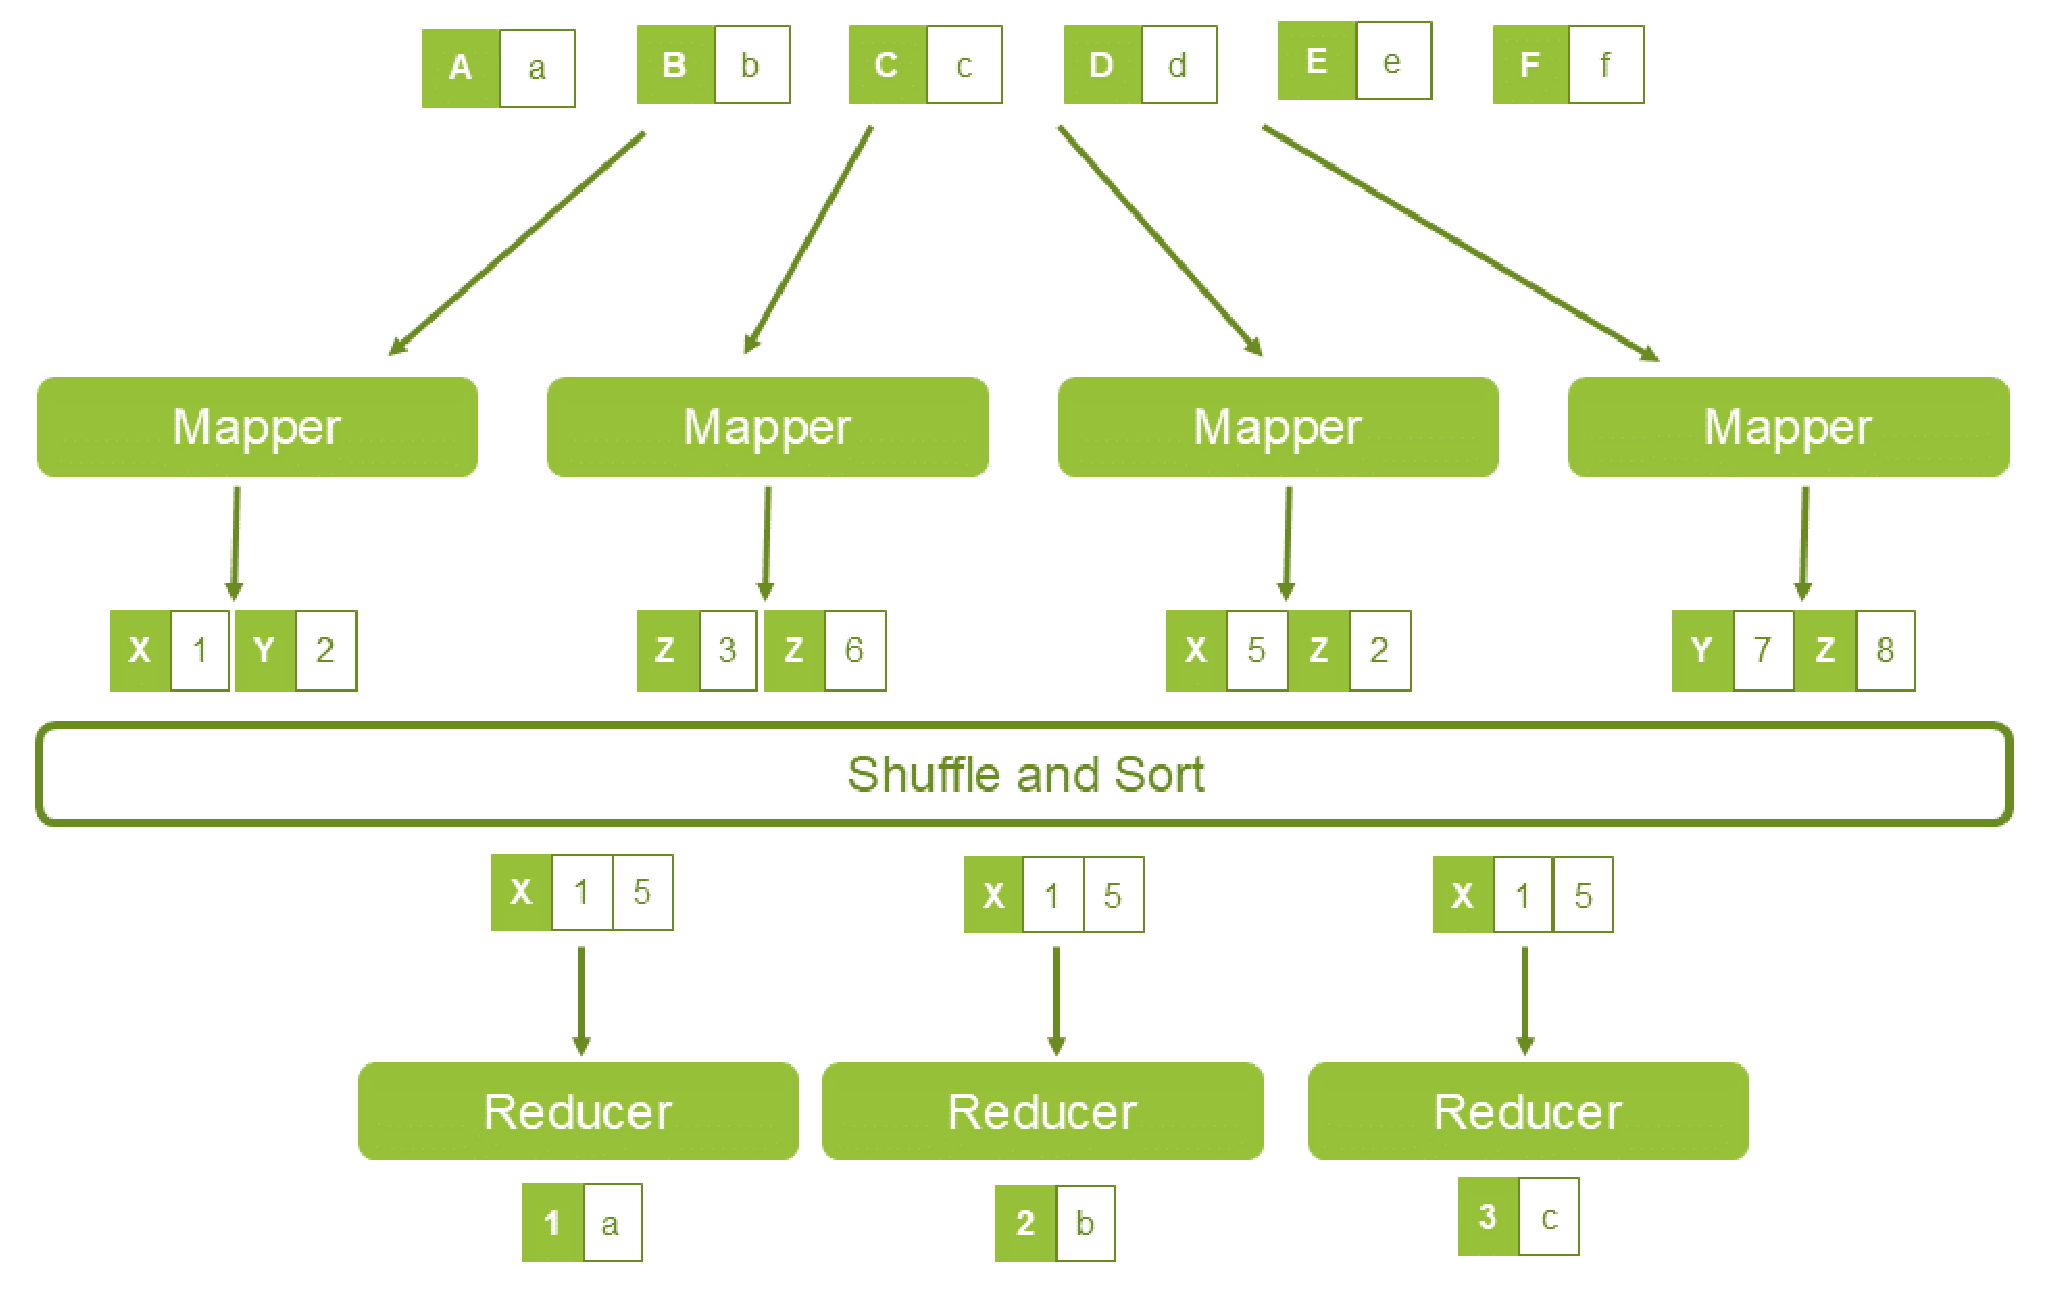
\includegraphics[width=1 \linewidth]{Thesis/Figures/Slide58.pdf}
\caption{\label{fig:MapReduce}MapReduce Programming
Model \cite{ketu2020performance}}
\end{figure}

The workflow of nodes in Hadoop is shown in \autoref{fig:hadoop}. Each MapReduce task is distributed across three nodes, the job submission node, the name node and the slave nodes, which ensure that the task is successfully completed. JobTracker and TaskTracker monitor the progress of the MapReduce tasks, while all operations are performed on DataNodes managed by the NameNode. These processes are executed within the slave nodes. \cite{ketu2020performance}

\begin{figure}[h]
\centering
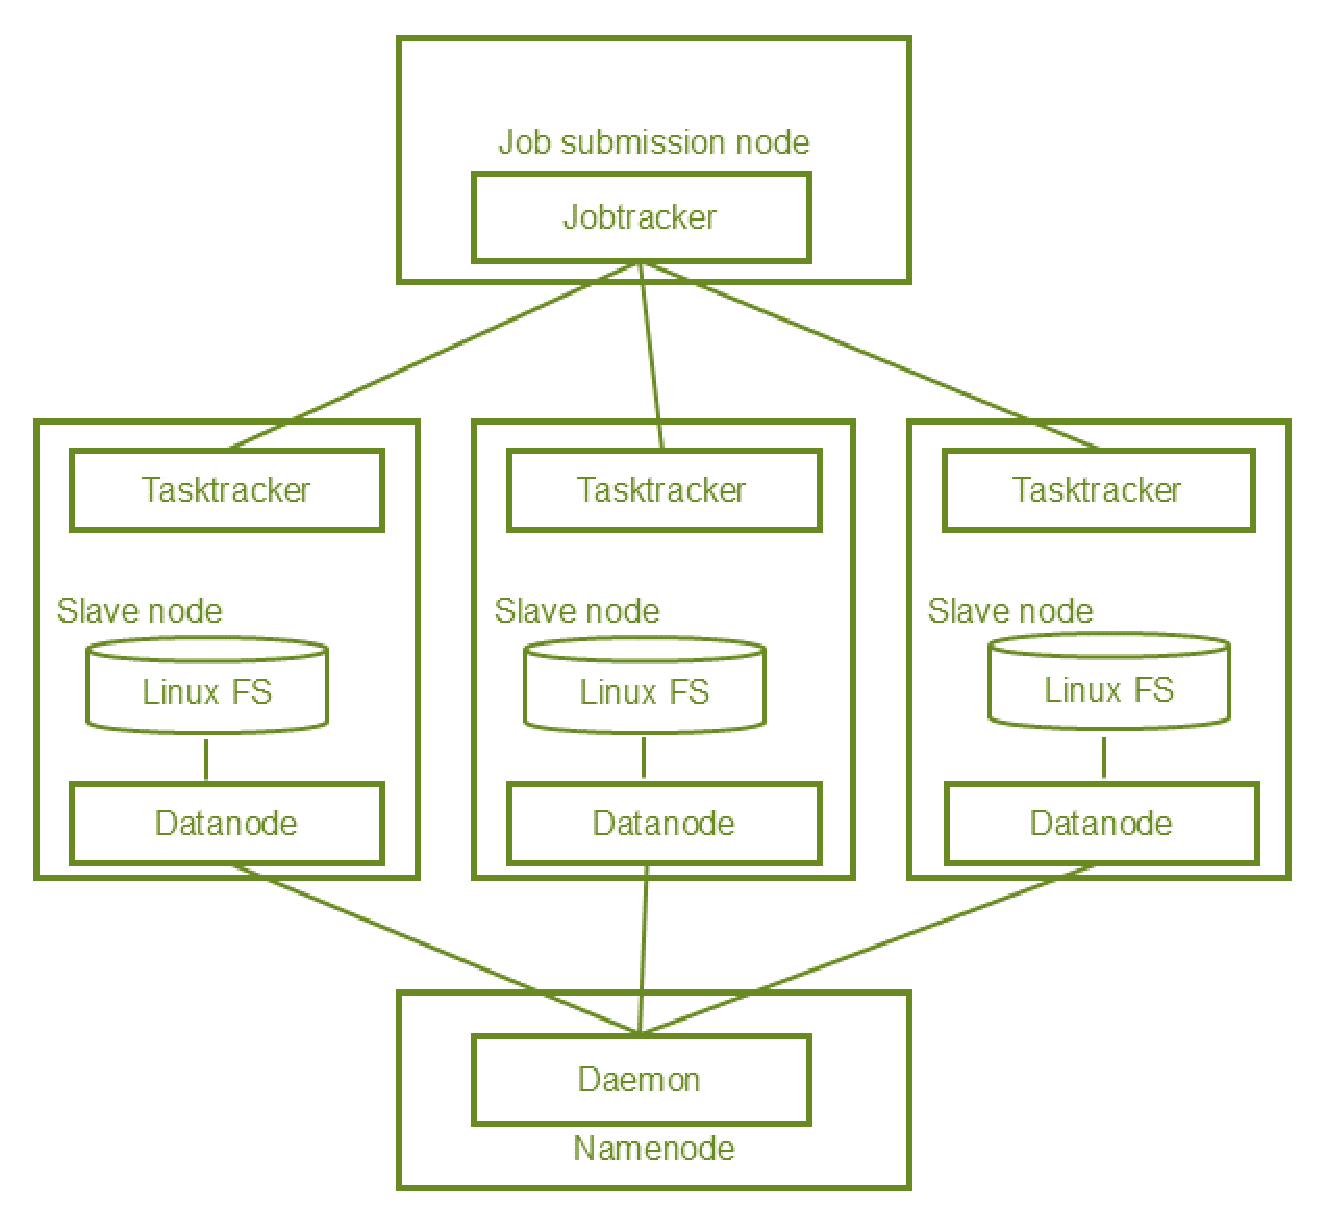
\includegraphics[width=1 \linewidth]{Thesis/Figures/Slide57.pdf}
\caption{\label{fig:hadoop}Node Work Flow in MapReduce Programming
Model \cite{ketu2020performance}}
\end{figure}

\subsection{Spark}

Apache Spark is a big data analytics framework based on distributed processing designed specifically for real-time data processing. Unlike Hadoop, which is based on disk-based computing, Spark uses in-memory computing, which significantly increases its processing speed. Spark supports multiple programming languages, including Python, Java and Scala and allows algorithms to be developed using any of these languages, unlike Hadoop, which relies on a single programming model. Spark also includes several specialised libraries, such as MLlib for machine learning, Spark SQL for structured data management and GraphX for graph processing. It supports parallel application development through Spark Streaming, which allows both real-time and batch data to be processed efficiently and quickly. \autoref{fig:spark} provides an overview of the Spark framework and its integration with higher-level tools and APIs. Core Spark is built on top of resilient distributed datasets \abk{RDD}{Resilient Distributed Datasets}, which can be sourced from internal storage such as HDFS, external storage, or created by other RDDs. These RDDs are managed using various storage options, including on-disk storage, in-memory serialised data and in-memory deserialised Java objects. \cite{ketu2020performance}

\begin{figure}[h]
\centering
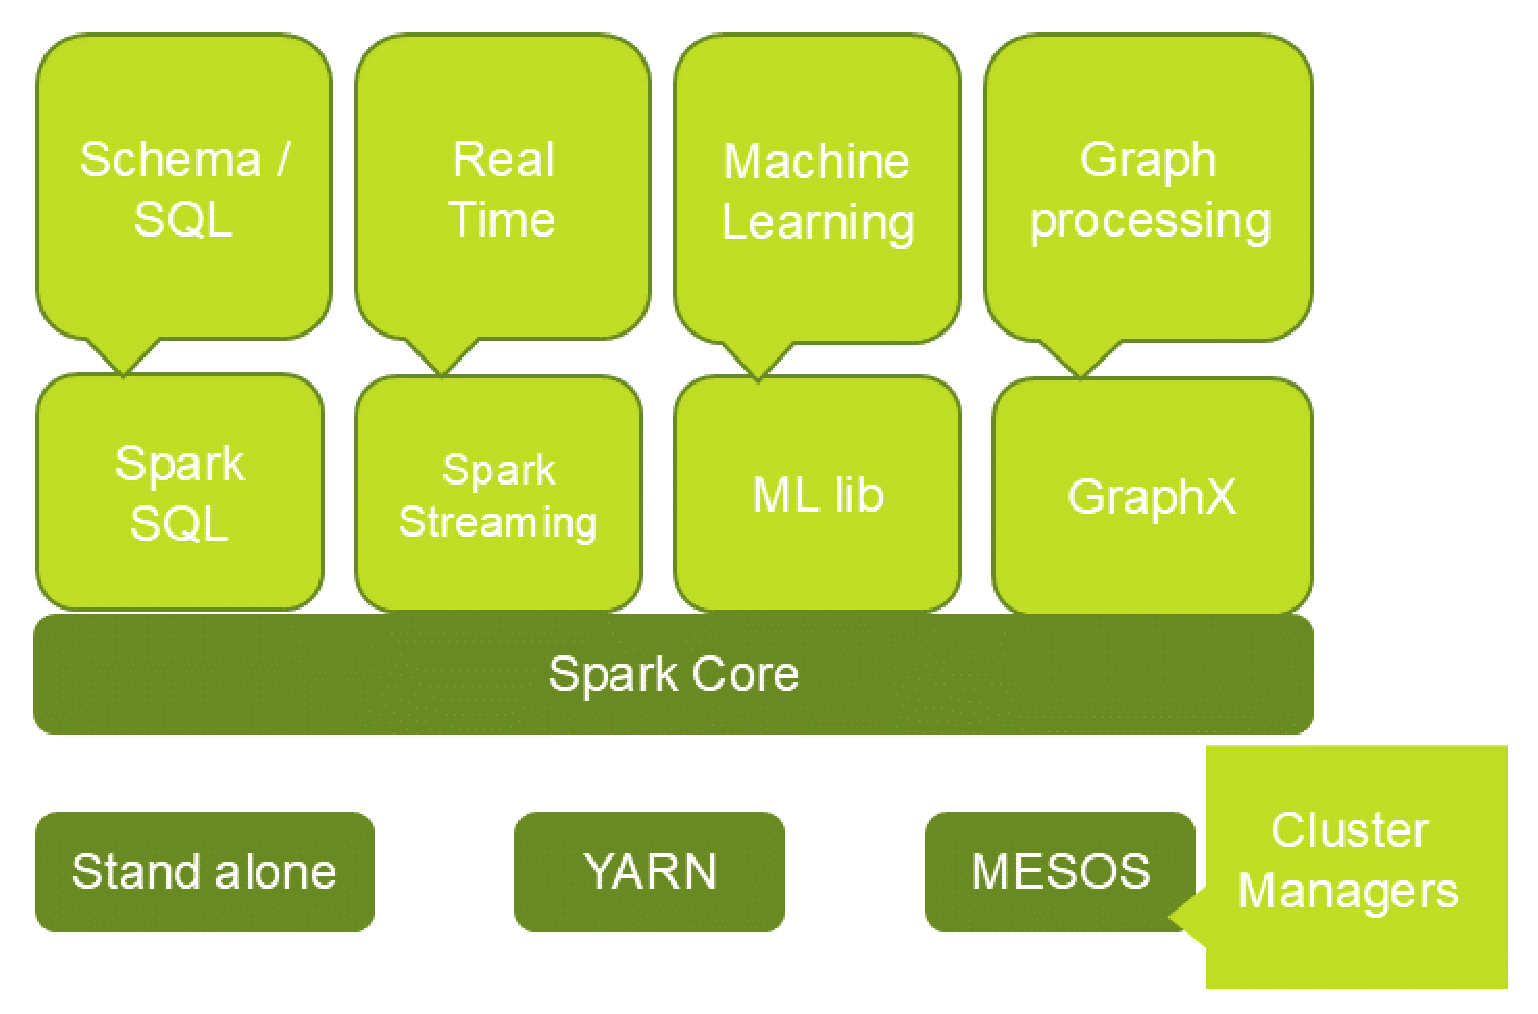
\includegraphics[width=0.8 \linewidth]{Thesis/Figures/Slide56.pdf}
\caption{\label{fig:spark}Spark Framework \cite{ketu2020performance}}
\end{figure}

Apache Spark provides stream processing capabilities through micro batching, where data streams are broken into small batches that are processed by Spark batch engine. While this approach is effective, it can still vary in performance compared to true stream processing frameworks. Spark is known for its unique features such as speed, ease of use, advanced analytics, in-memory computing and real time stream processing. It is exceptionally fast, up to 100 times faster than Hadoop and 10 times faster than disk based data access. It supports for multiple programming languages, making it easy for developers to use. Spark goes beyond basic map and reduce operations to support advanced analytics such as SQL queries, data streaming, machine learning and graph algorithms. It is highly flexible, running on different platforms such as Hadoop YARN, Mesos, EC2, Kubernetes, or as a standalone cluster in the cloud. Spark in-memory computing also enables iterative machine learning and complex data analysis at high speeds by keeping data in-memory. \cite{shaikh2019apache}

\subsection{Modin}

Modin is a framework designed to improve the performance of Pandas operations by enabling parallel execution with minimal changes to existing code bases. By simply modifying an import statement, users can take advantage of Modin optimizations to handle larger datasets more efficiently. The core of Modin architecture is to mimic the Pandas dataframe API while using parallel execution engines such as Ray or Dask as shown in \autoref{fig:modin}. \cite{shi2021leveraging}

\clearpage 

\begin{figure}[h]
\centering
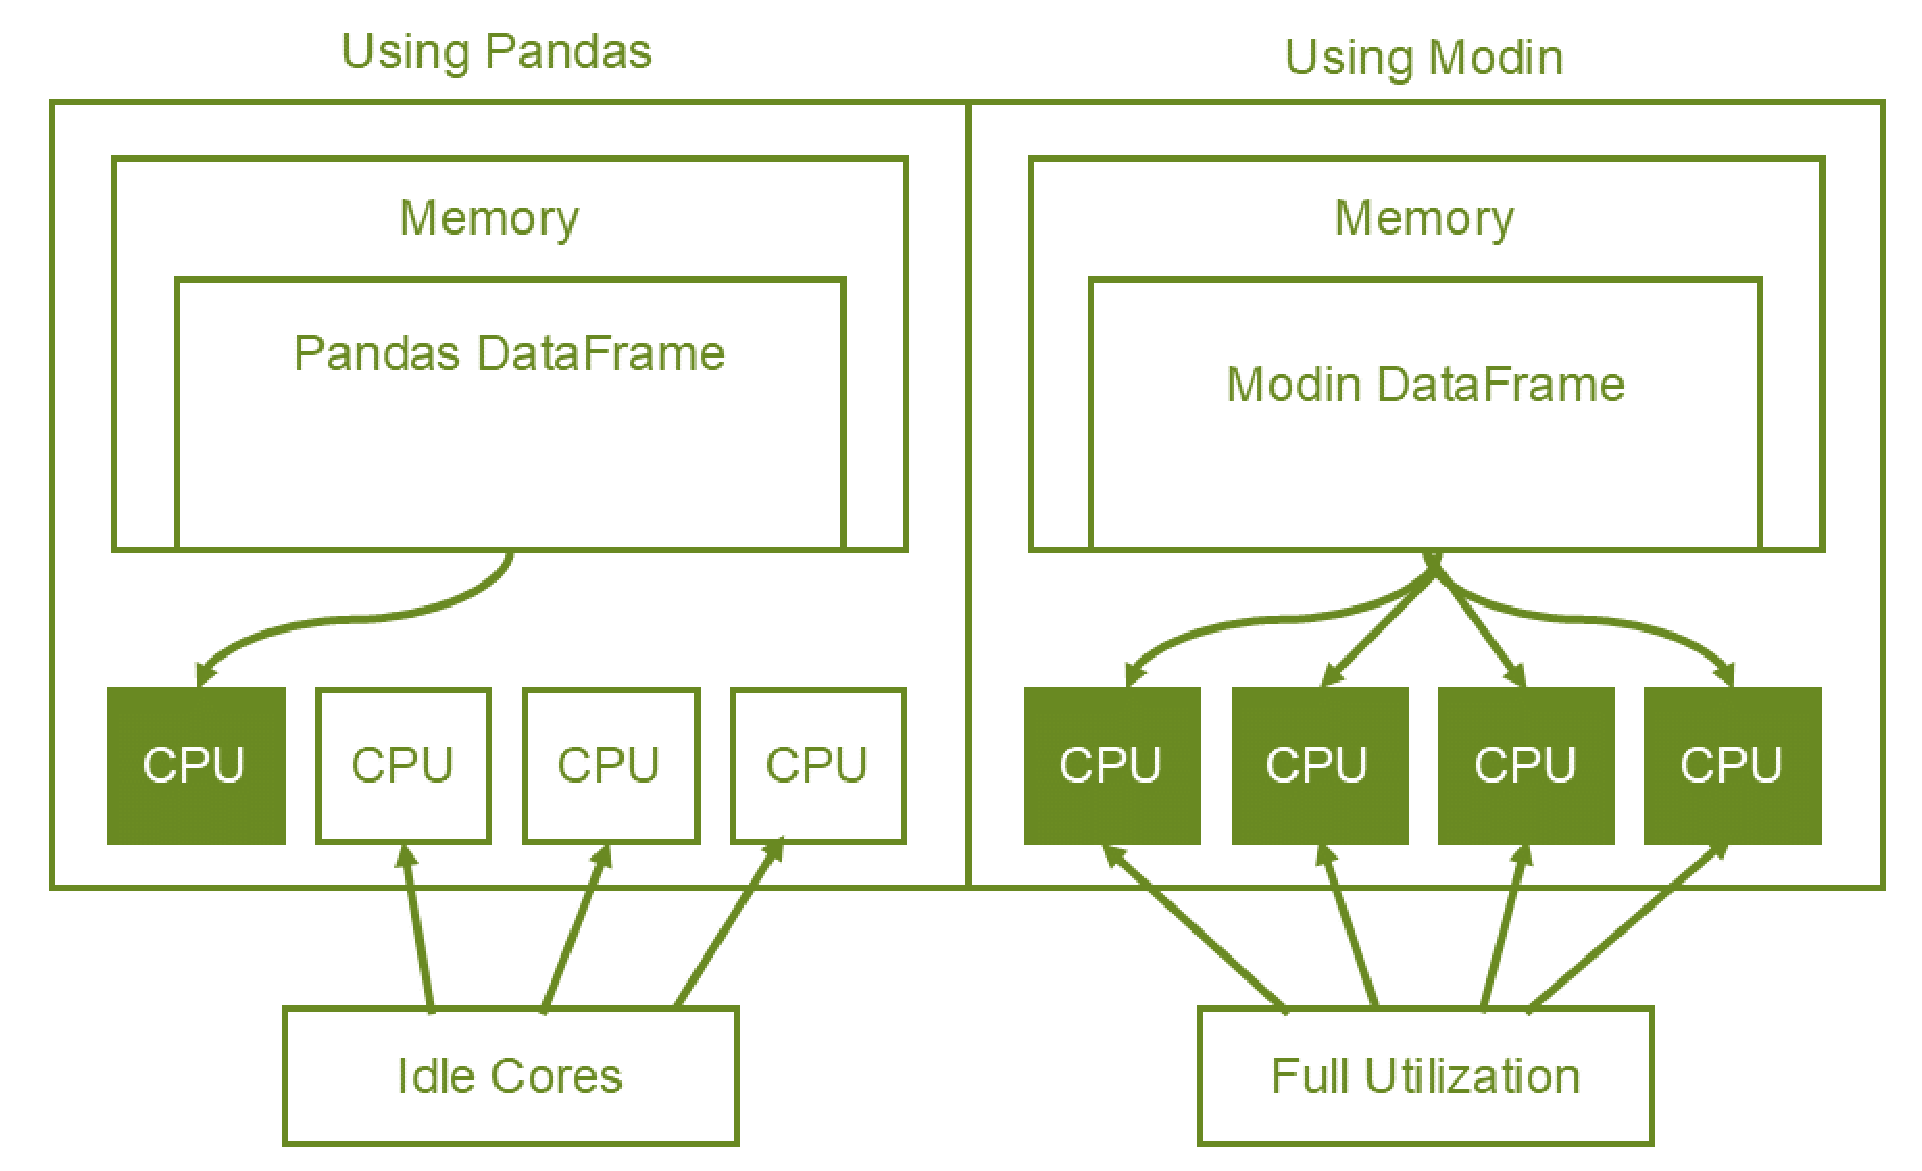
\includegraphics[width=1 \linewidth]{Thesis/Figures/Slide62.pdf}
\caption{\label{fig:modin}Modin Framework \cite{shi2021leveraging}}
\end{figure}



This allows Modin to translate high-level dataframe operations into a simplified set of basic algebraic operators such as select, join and map, making query planning and optimization easier. The traditional approach to Modin is eager execution, where queries are processed immediately as shown in \autoref{fig:eager modin}. \cite{shi2021leveraging}



\begin{figure}[h]
\centering
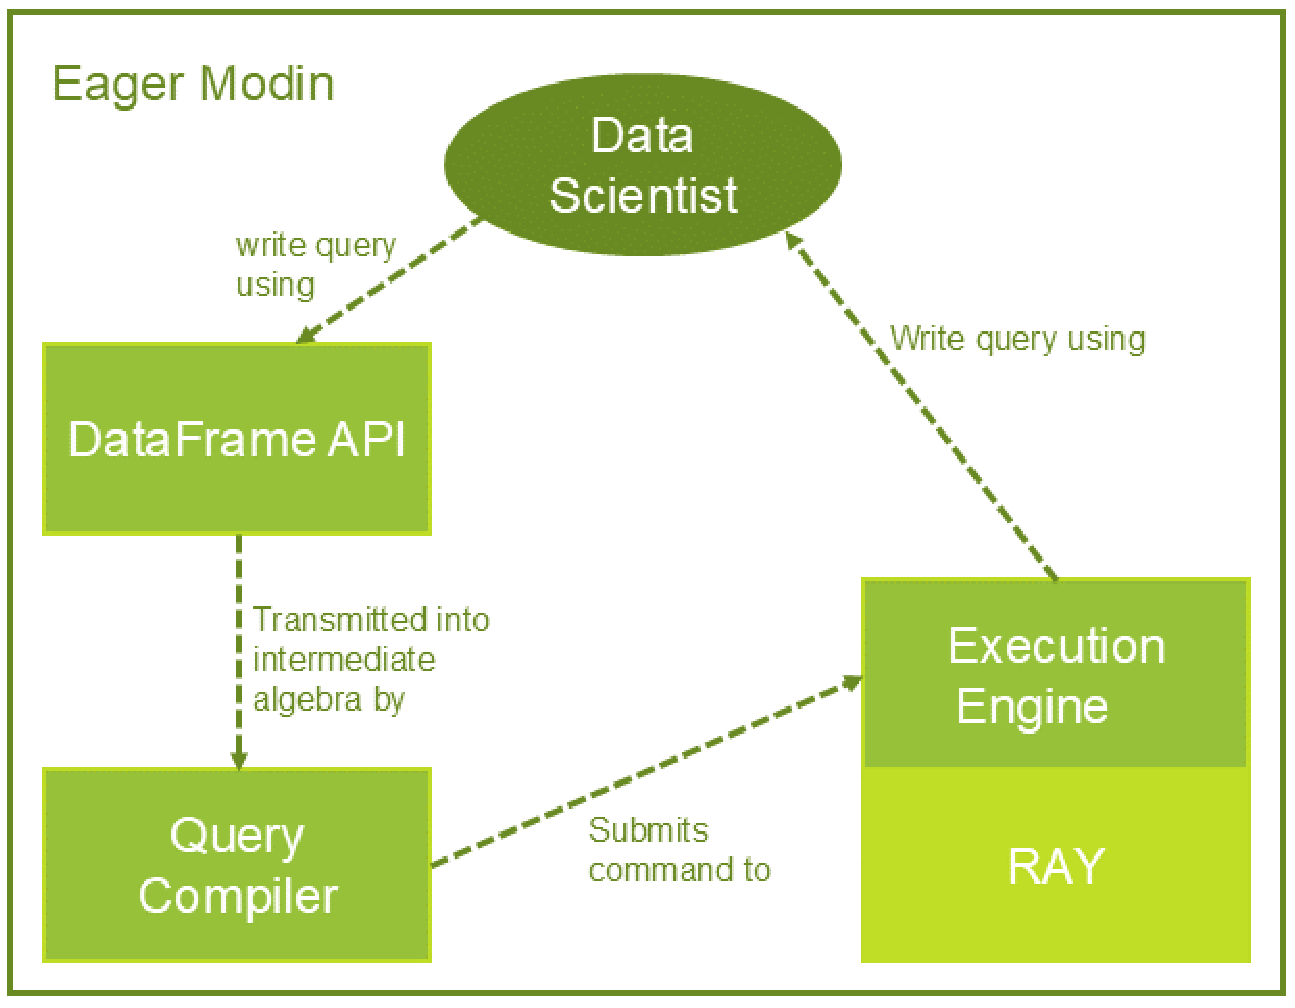
\includegraphics[width=0.8\linewidth]{Thesis/Figures/Slide64.pdf}
\caption{\label{fig:eager modin}Eager Modin Approach \cite{shi2021leveraging}}

\vspace{-20cm}
\end{figure}

\clearpage

However, New features of Modin include support for lazy execution, which delays query execution until explicitly requested by the user. This lazy approach allows optimization of query planning and collection of statistics during the users \texttt{think time} in interactive environments such as Jupyter notebooks, illustrated in \autoref{fig:lazy modin}. The underlying data in Modin dataframes is immutable and operations that appear destructive are implemented as copy on write, ensuring that the lazy execution framework handles updates efficiently. \cite{shi2021leveraging}



\begin{figure}[h]
\centering
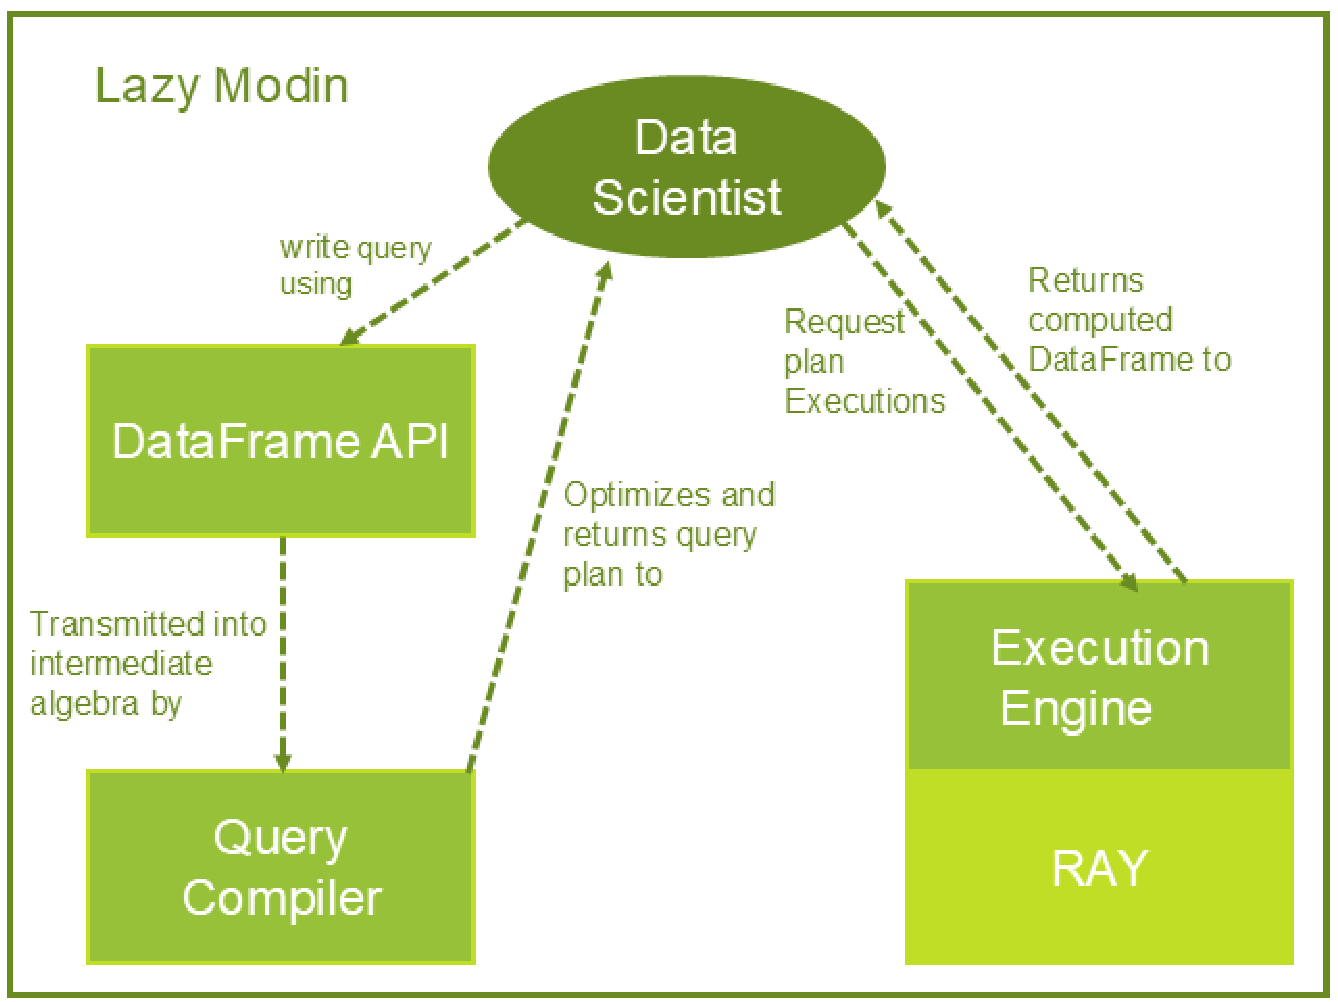
\includegraphics[width=0.8 \linewidth]{Thesis/Figures/Slide63.pdf}
\caption{\label{fig:lazy modin}Lazy Modin Approach \cite{shi2021leveraging}}
\end{figure}


\subsection{Dask}

Dask is a Python based big data engine that is gaining popularity for its ability to efficiently handle large-scale data processing tasks. Similar to Apache Spark, Dask uses in-memory computing, data locality and lazy evaluation to minimize unnecessary data transfers and computation. Dask workflows also take advantage of multithreading, allowing parallel processing when not constrained by Python global interpreter lock \abk{GIL}{Global Interpreter Lock}. Unlike Spark, which relies on coarse grained operations, Dask achieves fault tolerance through data lineage without this requirement, making it more flexible and modular. This modularity means that users can install only the components they need, keeping the system lightweight. Dask offers collection five main data structures tailored to different types of computation, Array, Bag, Dataframe, Delayed and Futures as shown in \autoref{fig:dask}. \cite{dugre2019performance}

\clearpage

\begin{figure}[h]
\centering
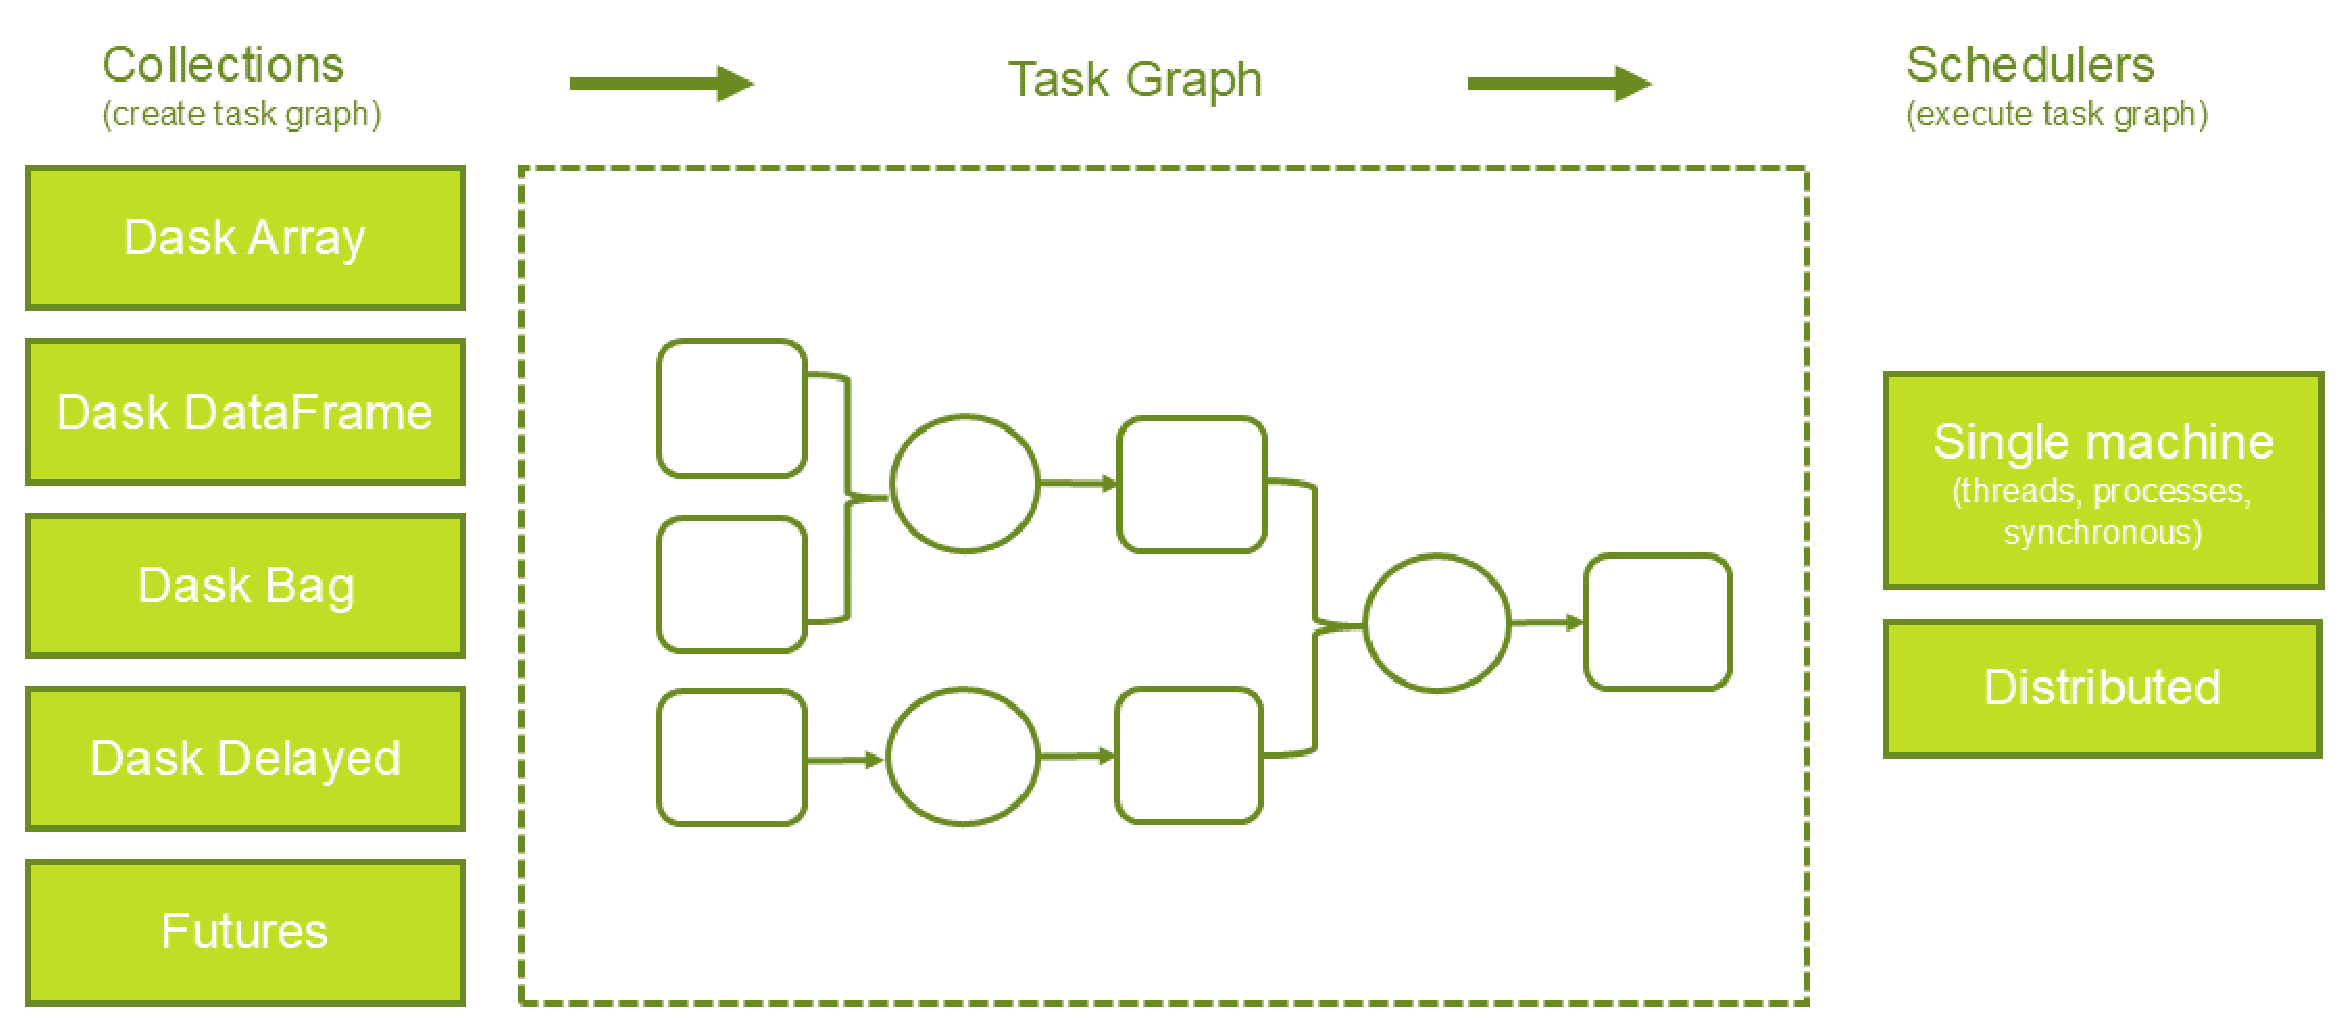
\includegraphics[width=1 \linewidth]{Thesis/Figures/Slide61.pdf}
\caption{\label{fig:dask}Dask Framework \cite{dask_docs}}
\end{figure}

Dask Array is designed for processing large numerical arrays and works as a distributed version of NumPy. Dask Bag, similar to Spark RDD, handles collections of Python objects and provides a parallel abstraction similar to the PyToolz library. The Dask dataframe allows parallel processing of large tabular datasets by distributing computations across multiple Pandas dataframes as shown in \autoref{fig:dask frame}. Dask Delayed is used to define custom tasks that don't fit into the other structures and supports lazy execution. In contrast, Dask Futures also handle arbitrary tasks, but operate in real time rather than waiting to be triggered. Most Dask structures use a local multi threaded scheduler by default, while Dask Bag specifically uses a multi processing scheduler. \cite{dugre2019performance}

\begin{figure}[h]
\centering
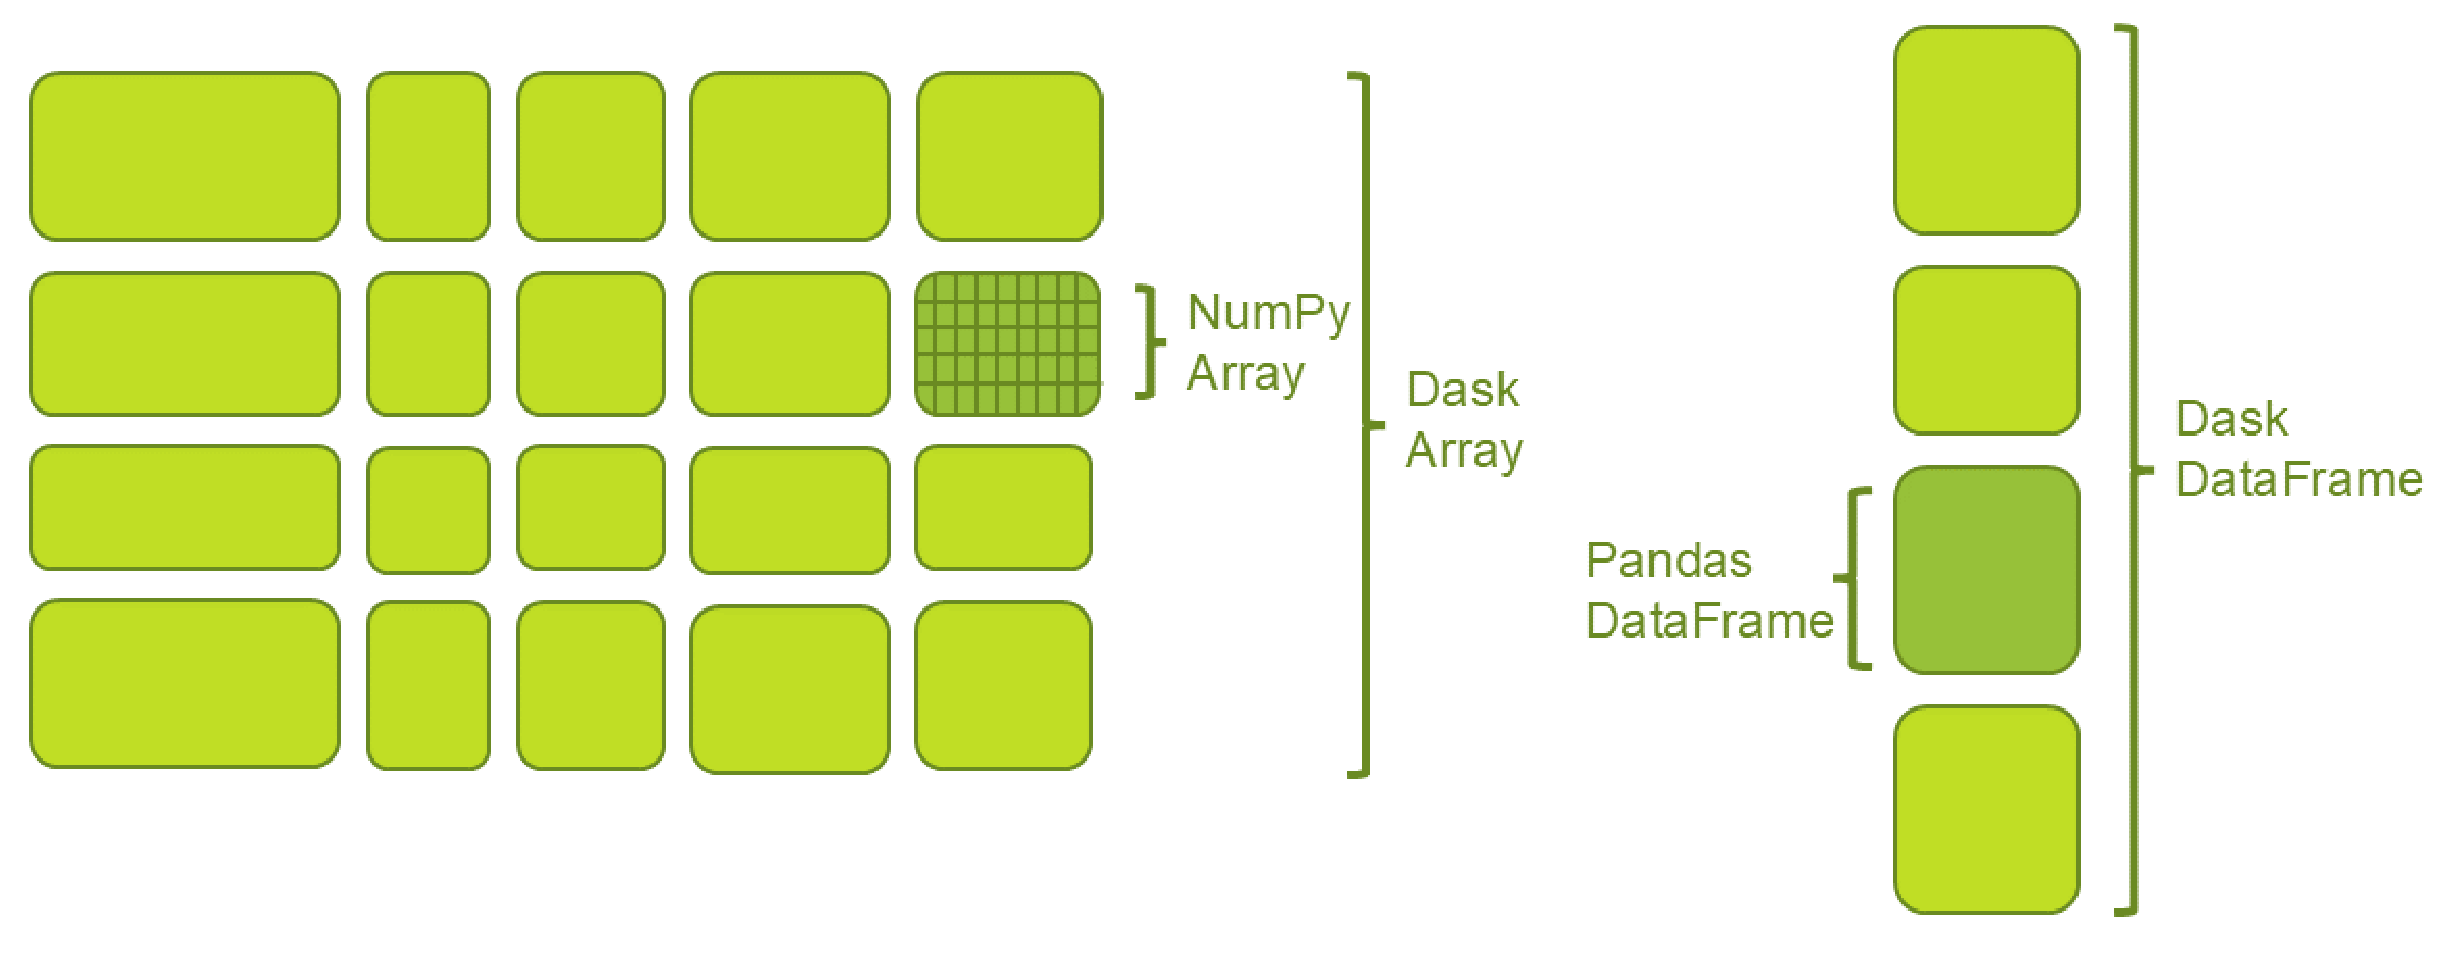
\includegraphics[width=1 \linewidth]{Thesis/Figures/Slide60.pdf}
\caption{\label{fig:dask frame}Dask Dataframe \cite{dask_docs}}
\end{figure}

\clearpage

\subsection{Optuna}

Optuna is an automated hyperparameter optimization framework designed specifically for machine learning. It offers a flexible API, define by run style, that enables user high modularity and dynamic construction of search spaces, thus providing a robust and adaptable solution for hyperparameter optimization of ML or DL models. Its lightweight, flexible and platform agnostic architecture enables the support of a wide range of tasks with minimal installation requirements. Optuna permits users to define search spaces in accordance with familiar Python syntax, including conditionals and loops. Furthermore, it employs algorithms to efficiently sample hyperparameters and prune unpromising trials and it facilitates straightforward parallelization, allowing studies to be scaled to encompass dozens or hundreds of workers with minimal code modifications as shown in \autoref{fig:optuna}. It also provides rapid visualization tools for the inspection of optimization histories through a variety of plotting functions. The framework is centered upon two principal concepts, first one is \texttt{study}, which represents an optimization based on an objective function and second is \texttt{trial}, which denotes a single execution of the objective function. \cite{optuna_docs}

\begin{figure}[h]
\centering
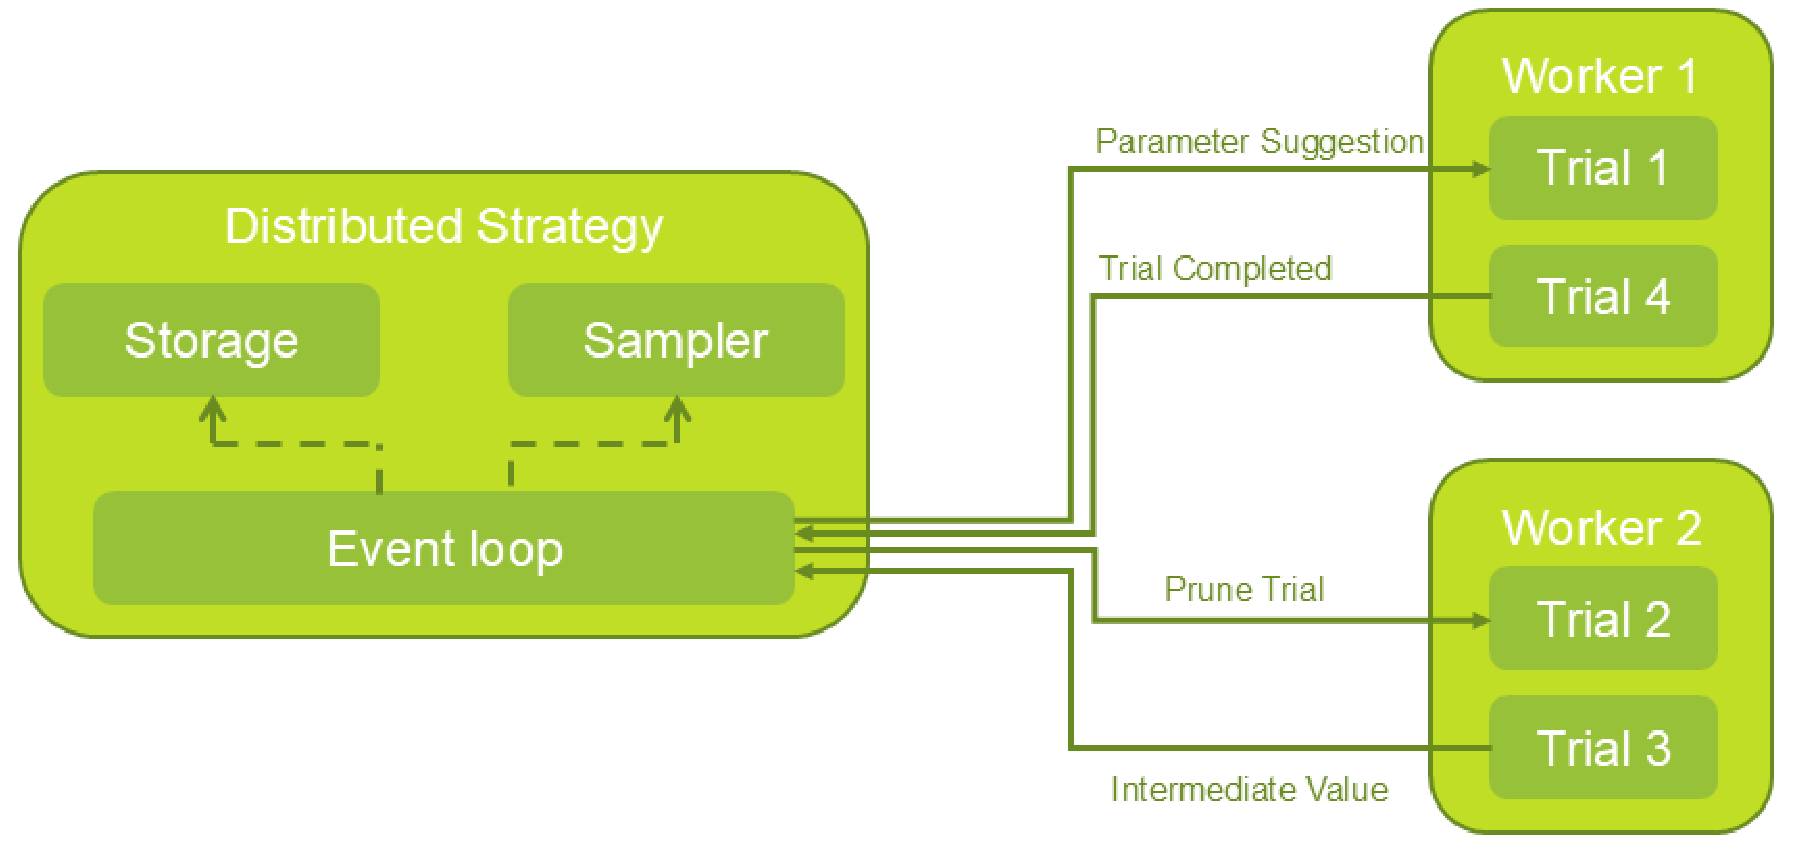
\includegraphics[width=1 \linewidth]{Thesis/Figures/Slide65.pdf}
\caption{\label{fig:optuna}Optuna Tuning Architecture \cite{optuna_hpo}}
\end{figure}

\subsection{TensorFlow}

TensorFlow is an open source library developed by Google for large-scale ML and DL tasks. It simplifies the development, training and optimization of machine learning models by combining computational algebra and optimization techniques. TensorFlow is highly efficient at performing complex mathematical calculations that are essential for ML and it uses tensors multi-dimensional arrays to encode data in ML or DL models. A key feature of TensorFlow is its ability to design data flow graphs, where data flows through a series of processing nodes, making it highly scalable and flexible across platforms such as cloud, mobile, desktop and web. TensorFlow provides two level of APIs low-level and high-level. Developer uses low-level APIs to build custom ML models and beginners uses high-level APIs which allows to interact with pre-built ML capabilities. TensorFlow architecture follows a simple three step process shown in \autoref{fig:TensorFlow}, the first being data preprocessing, which involves reading and transforming data for the model, then building the model and finally training, which uses optimization techniques such as back propagation to improve model accuracy and estimate model performance. TensorFlow serving is an important component of TensorFlow library, which is used to deploy ML models in production environment. It allows to have multiple versions of a model, which are called servables and can be deployed, updated and managed over a period of time. These servables can be created from lookup tables or complete models and can be deliver through streams of servable versions. The load of these servables is manged by TensorFlow source, to ensure smooth transitions between versions during serving. In addition, TensorFlow provides a highly, scalable and optimised environment developing, training and deploying ML models. \cite{ramchandani2022survey}

\begin{figure}[h]
\centering
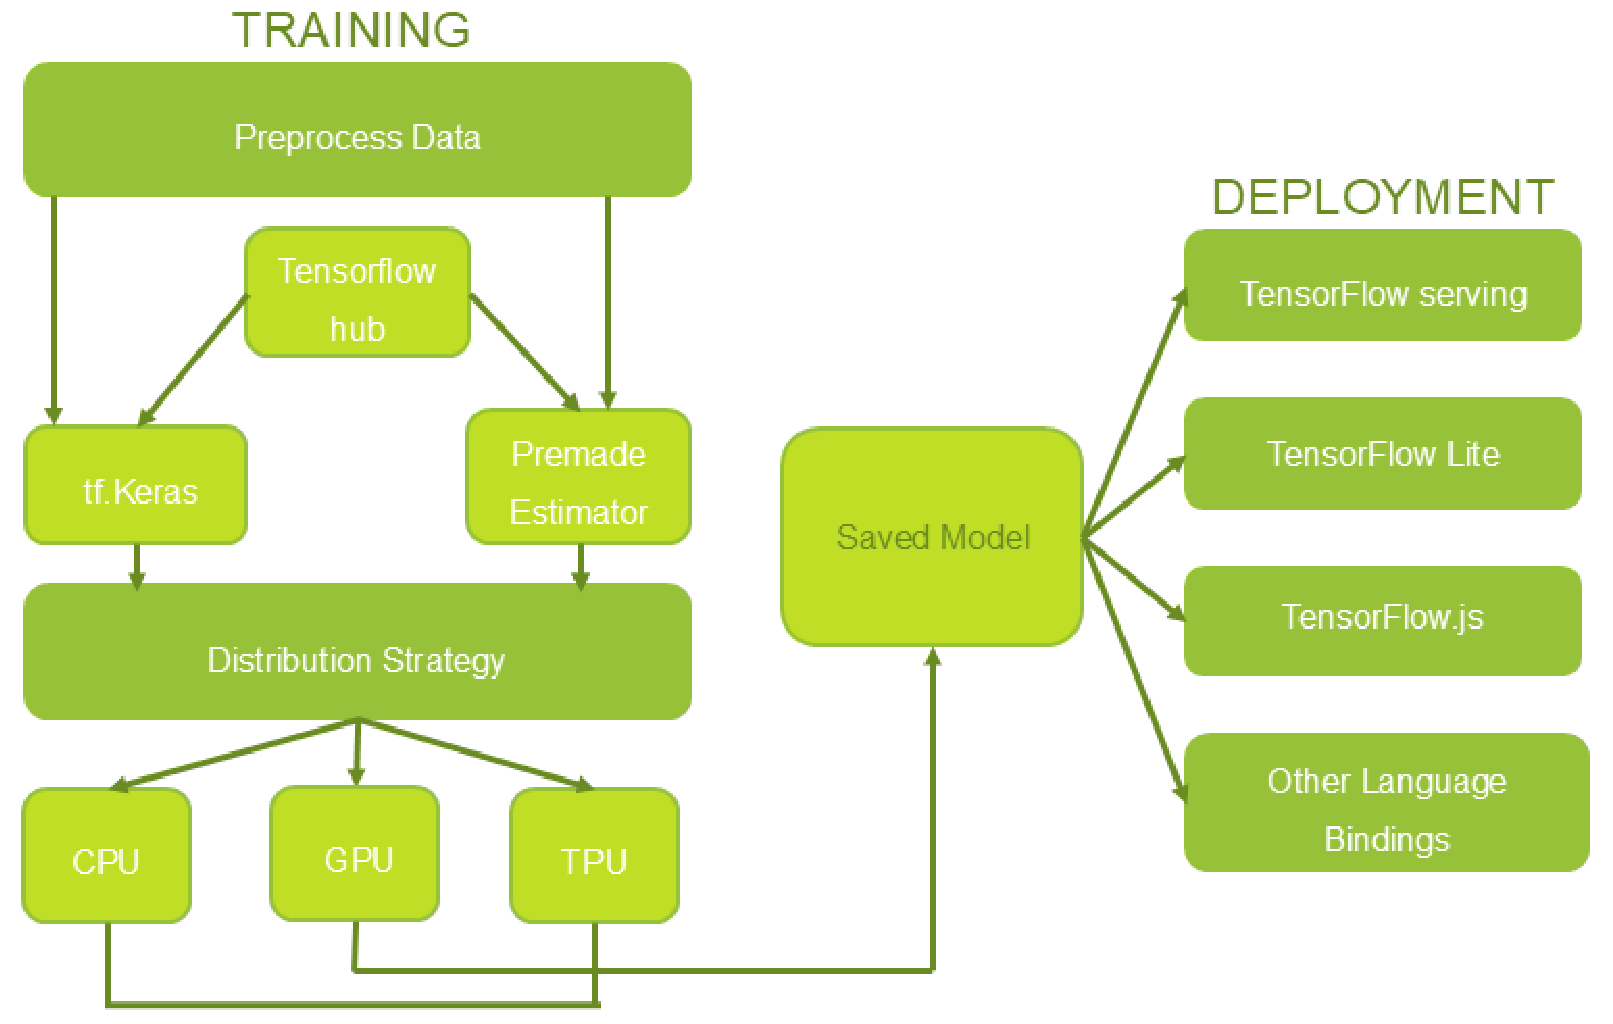
\includegraphics[width=1 \linewidth]{Thesis/Figures/Slide66.pdf}
\caption{\label{fig:TensorFlow}TensorFlow Architecture \cite{ramchandani2022survey}}
\end{figure}

\subsection{Hyperopt}

Hyperopt is a library for optimising hyperparameters for algorithm configuration, especially in ML models. It handles complex search spaces that can include different types of variables such as continuous, ordinal and categorical, different sensitivity profiles such as uniform versus logarithmic scaling and conditional structures where different parameters become relevant depending on which classifier is chosen. As shown in \autoref{fig:Hyperopt}, the optimisation process involves several key steps. Data transformation is the first step, which prepares the raw data through preprocessing techniques such as normalisation or principal component analysis \abk{PCA}{Principal Component Analysis}. The second step is model selection, which involves choosing the appropriate ML models for the transformed data. The last step is hyperparameter optimisation. This involves defining a search domain where the hyperparameters are treated as random variables, specifying an objective function to evaluate model performance and using an optimisation algorithm (e.g. TPE) to explore the search space. Integration with scikit-learn facilitates model training and validation, while Hyperopt-sklearn extends these capabilities by handling complex pipelines of preprocessing steps and models. It also manages conditional hyperparameters and uses blacklist rules to ensure efficient and valid optimisation. \cite{komer2014hyperopt}


\begin{figure}[h]
\centering
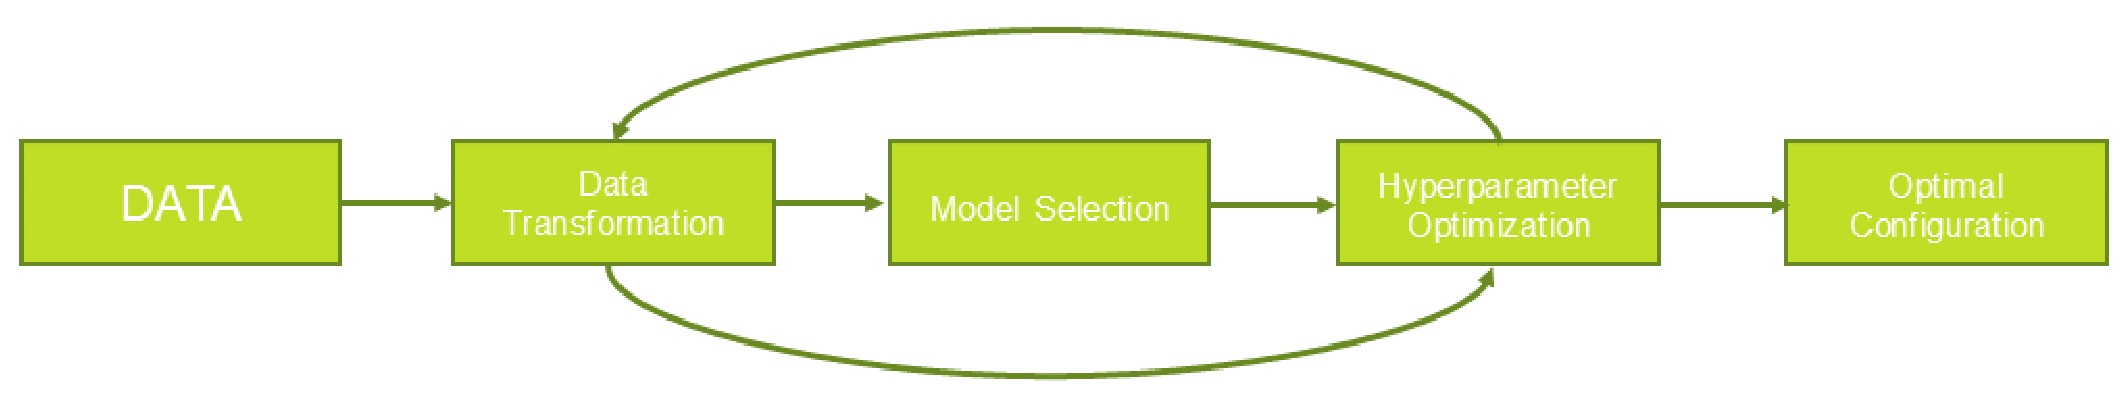
\includegraphics[width=1 \linewidth]{Thesis/Figures/Slide67.pdf}
\caption{\label{fig:Hyperopt}Hyperopt Tuning \cite{hyperopt_bayesian_optimization}}
\end{figure}


\section{Comparison Criteria}

To evaluate Ray against other distributed computing tools such as Apache Spark, Dask, Modin, Optuna, Hyperopt and TensorFlow, several criteria are considered. These criteria focus on key aspects that influence the selection of a distributed computing framework based on specific use cases, including the following.

\begin{itemize}
    \item Scalability
    \item Performance
    \item Flexibility
    \item Cost
    \item Compatibility
    \item Ease of use
    
\end{itemize}

The ability of a distributed computation framework to be scaled up or down is a crucial criterion for selecting the appropriate framework, as it determines the systems ability to be economically deployed across a wide range of sizes and configurations. A scalable framework must achieve an effective balance between cost and performance, with effectiveness measured in terms of through-put and quality of service. The scalability of a system is measured by how well it performs across different sizes or levels, based on a specific metric that combines the original design and the scaling strategy. A good scaling strategy adjusts the system systematically as it grows, often using automated design optimization at each step. Efficient scaling shows how well the system is designed and helps identify areas for improvement, ensuring it can handle changing demands while maintaining good performance. Therefore, selecting a distributed computation framework with proven scalability ensures adaptability and performance across different operational scales. \cite{jogalekar2000evaluating}

Performance refers to the response time or throughput observed by the end user. It's common for distributed systems to not meet their performance goals when they are first built. Some systems work well with a small number of users, but lack the scalability to accommodate increased usage. Poor performance can lead to several negative outcomes, such as damaging customer relationships, reducing user productivity, losing revenue, increasing costs for fixing or redesigning the system and missing out on market opportunities in a timely manner. The majority of performance failures is due to lack of consideration on performance issues at an early stage of the development process, particularly within the architectural phase. It is therefore essential that a distributed computing framework is designed in a way that ensures the system's performance is consistently reliable, scalable and capable of meeting the demands of increasing workloads. It is of the utmost importance to consider performance issues at the architectural design phase, including factors such as synchronization mechanisms, resource allocation and load balancing. This will prevent future performance bottlenecks and ensure that the system can scale effectively as usage grows. \cite{smith2002performance}

The ability of distributed computing framework to adapt changing infrastructure is important factor in the selection of distributed computing framework. The flexibility of the infrastructure allows computing loads to be balanced on the fly as more users join the system. The process of setting up the infrastructure has become so standardised that adding computing resources has become almost as simple as adding building blocks to an existing grid. Flexibility in distributed computing framework is also important because, it helps to manage the different workloads efficiently. As the number of user increases, the system can more effectively balance the demand, making it easier to manage, while also benefiting from cost savings as it grows. Therefore, flexibility is essential to consider in order to achieve the distributed system that can dynamically adjust to changing demands while maintaining performance and avail benefits of scalability and resource optimization. \cite{avram2014advantages}

The cost of distributed computing framework considered as a significant criteria in selection of distributed computing framework, as it allow to execute large and complex processing task with minimum resources which make it accessible for smaller companies, which used to be available only to large organizations. This makes it a good choice for organizations looking to save cost both in terms of financially and computing resources. Furthermore, cloud computing frameworks enables the dynamic allocation of resources, which is beneficial for computational tasks that require computing power for relatively short periods of time. Affordability and scalability of resources makes cost a key factor in choosing a distributed computing framework for organization. \cite{avram2014advantages}

When selecting a distributed computing framework, compatibility is the important criteria, as it guarantees the easy of integration with current tools and technologies. Distributed systems is based on combination of different independent components or services. To work effectively with each other compatibility between components or resources is essential. The interaction protocols are used to determine how these components can communicate with each other and have a significant impact on their compatibility. The ability of a framework to follow these communication protocols and to integrate with different components or services reduces the need for extensive modifications and helps to avoid potential integration problems. Compatibility therefore not only simplifies implementation, but also increases the overall flexibility and scalability of distributed computing systems. \cite{chevrou2019modular}

When choosing a distributed computing framework, it is essential to prioritize ease of use. As this has a direct impact on developer productivity and efficiency. An easy to use framework simplifies the development process by providing intuitive APIs and clear abstractions. Allowing developers to focus on solving domain specific problems rather than managing complex distributed systems. The frameworks with well designed interfaces and extensive documentation reduce the time required to learn and deploy applications effectively. Prioritizing usability in the selection process ensures that distributed computing can be used effectively, maximizing both developer satisfaction and project success. \cite{zaharia2012resilient}.



\section{Comparison of Ray Core with Apache Spark and Dask}


The Ray core is discussed earlier in this report and provides primitive methods such as tasks, actors and objects that are used to develop scalable and distributed computing resources \cite{ray_doc}. \autoref{tab:table1} present a comparison of Ray core with Apache Spark and Dask, focusing on how these frameworks manage distributed computing tasks. The evaluation is based on criteria such as scalability, performance, flexibility, cost, compatibility and ease of use, which are essentials factors in distributed computing, particularly in the context of large-scale applications or big data processing.


\begin{table}[h]
\centering

\begin{tabular}{|p{2.6cm}|p{4cm}|p{4cm}|p{4cm}|}
\hline
\textbf{Feature} & \textbf{Ray Core} & \textbf{Apache Spark} & \textbf{Dask} \\
\hline
\textbf{Scalability} & Provide high scalability, can scale across many node and cores. \cite{ray_doc} & Provide high scalability for large-scale data. \cite{apache_spark}& Ability to scale is limited for large dataset \cite{dask_docs} \\
\hline
\textbf{Performance} & High performance with low overhead, efficient for distributed tasks. \cite{ray_doc} & High performance, due to in-memory processing but have higher latency due to disk based storage \cite{apache_spark}&Good performance, for Python based tasks, but need tuning for large-scale use. \cite{dask_docs} \\
\hline
\textbf{Flexibility} & supports various distributed computing paradigms including task and actor models. \cite{ray_doc}& Flexible with rich APIs, supports many data formats. \cite{apache_spark}& Modular design allow users to install only the required components. \cite{dugre2019performance}\\
\hline
\textbf{Cost} & Cost effective, require dedicated resources for monitoring, scaling and handling failures. \cite{ray_doc} & Operational cost overhead including monitoring, scaling and handling failures. \cite{apache_spark}& Cluster involves operational overhead, including monitoring and optimizing performance. \cite{dask_docs}\\
\hline
\textbf{Compatibility} & Support Python and integration with other Ray libraries for diverse workflows. \cite{ray_doc} & Support Python, R and Scala \cite{apache_spark}& Integrate easily with Python libraries and workflows. \cite{dask_docs} \\
\hline
\textbf{Ease of Use} & Easy to use for Python developers, very well documented. & Multi language support make it suitable for majority of developers. & User friendly for Python developer\\
\hline
\end{tabular}
\caption{Comparison of Ray Core, Apache Spark and Dask Features}
\label{tab:table1}
\end{table}

\section{Comparison of Ray Data with Apache Spark and Modin}


Ray Data was discussed in the previous chapter as a tool that facilitates distributed data processing and integrates seamlessly into ML workloads \cite{ray_doc}. In this section, Ray Data is compared to other popular distributed data processing tools to assess its strengths and weaknesses. The \autoref{tab:table2} provides a comparative analysis of Ray Data, Apache Spark and Modin across several important dimensions like scalability, performance, flexibility, cost, compatibility and ease of use. In context of Ml workloads, scaling APIs and Data Processing.

\begin{table}[ht]
\centering
\begin{tabular}{|p{3cm}|p{3.5cm}|p{3.5cm}|p{3.5cm}|}
\hline
\textbf{Feature} & \textbf{Ray Data} & \textbf{Apache Spark} & \textbf{Modin} \\
\hline
\textbf{Scalability} & Highly scalable for distributed workloads with dynamic task distribution across nodes. \cite{ray_doc}& Highly scalable and optimized for batch processing. \cite{apache_spark} & Provide scalability with Ray backend, suitable for dataframe operations. \cite{modin_docs} \\
\hline
\textbf{Performance} & Suitable for both small and large-scale data processing. \cite{ray_doc} & High performance, optimize memory usage can avoid memory errors. \cite{apache_spark}& High performance for large dataset, which even cannot fit in-memory. \cite{modin_docs}\\
\hline
\textbf{Flexibility} & Very flexible, supports various task, actor and models. \cite{ray_doc}& Vast ecosystem have many data processing option. \cite{apache_spark} &Flexible approach in dataframe operation. \cite{modin_docs} \\
\hline
\textbf{Cost} & Fast and cheap for ML applications. \cite{ray_doc}& Can be costly when scaling resources. \cite{apache_spark}& Cost effective but scales with the size of the data and operation. \cite{modin_docs} \\
\hline
\textbf{Compatibility} & Integrates well with TensorFlow, PyTorch and other libraries. \cite{ray_doc}& Broad compatibility with data formats and resources. \cite{apache_spark} & Compatible with Pandas and Python tools. \cite{modin_docs} \\
\hline
\textbf{Ease of Use} & Easy to use for Python developers, very well documented. & Require knowledge of Spark APIs. \cite{apache_spark}& Easy to use Pandas like APIs. \cite{modin_docs} \\
\hline
\end{tabular}
\caption{Comparison of Ray Data, Apache Spark and Modin Features}
\label{tab:table2}
\end{table}

\clearpage

\section{Comparison of Ray Train with Apache Spark and Dask}


Ray Train is a distributed training library within the Ray ecosystem designed to facilitate large-scale ML models by enabling efficient training across multiple GPUs or nodes. In this section, Ray train in is evaluated against Apache Spark and Dask, highlighting its strengths and weaknesses relative to these popular distributed computing frameworks. \autoref{tab:table3} provides a comparative analysis across several important dimensions like scalability, performance, flexibility, cost, compatibility and ease of use. These criteria are critical when evaluating tools for scaling and distributed training. \cite{ray_doc}

\begin{table}[ht]
\centering
\begin{tabular}{|p{2.5cm}|p{3.8cm}|p{3.3cm}|p{3.8cm}|}
\hline
\textbf{Feature} & \textbf{Ray Train} & \textbf{Apache Spark} & \textbf{Dask} \\
\hline
\textbf{Scalability} & Highly scalable ML libraries for distributed training. \cite{ray_doc} & Offer manual optimization of memory caching, which provide high scalability while training. \cite{garcia2017comparison}& Provide Dask cluster to parallelize workload on many machines to train ML models. \cite{dask_docs}\\
\hline
\textbf{Performance} & High performance for distributed training tasks and workflows. \cite{ray_doc} & Provide iterative computation, enabling MLlib to run fast \cite{apache_spark} & Provide Dask scheduler to understand the characteristics of computations. \cite{dask_docs}\\
\hline
\textbf{Flexibility} & Provide support for frameworks like PyTorch, TensorFlow, XGBoost and many others. \cite{ray_doc} & Provide interoperating with libraries like NumPy and R. \cite{apache_spark} & Allows to deploys XGBoost alongside Dask. \cite{dask_docs}\\
\hline
\textbf{Cost} & Cost effective due to dynamic scaling using actors. \cite{ray_doc}& Perform fast distributed computing using in-memory primitives. \cite{garcia2017comparison} & Not able to cope with datasets larger then machine memory. \cite{dask_docs} \\
\hline
\textbf{Compatibility} & Provide ecosystem of API to interact with different training framework. \cite{ray_doc} & Compatible with Kubernetes, Hadoop, Apache Mesos, standalone, or in the cloud. \cite{apache_spark}& Compatible with Scikit-learn library for distributed training. \cite{dask_docs}\\
\hline
\textbf{Ease of Use} & Easy to use for Python developers, very well documented. & Require knowledge of NumPy, R and Spark APIs. \cite{apache_spark}& Easy to use for Python developers. \\
\hline

\hline
\end{tabular}
\caption{Comparison of Ray Train, Apache Spark and Dask Features}
\label{tab:table3}
\end{table}


\clearpage

\section{Comparison of Ray Tune with Optuna and Hyperopt}


Ray Tune is an advanced library within the Ray ecosystem that specializes in hyperparameter optimization for machine learning models. It uses Ray infrastructure to manage and execute tuning tasks across multiple nodes. Ray Tune supports a wide range of optimization algorithms and integrates seamlessly with ML frameworks, making it suitable for complex and large-scale tuning tasks. \autoref{tab:table4}, provide a comparison of Ray Tune with other popular tuning libraries to identify its benefits. \cite{ray_doc}



\begin{table}[ht]
\centering
\begin{tabular}{|p{3cm}|p{3.8cm}|p{3.8cm}|p{3.8cm}|}
\hline
\textbf{Feature} & \textbf{Ray Tune} & \textbf{Optuna} & \textbf{	Hyperopt} \\
\hline
\textbf{Scalability} & Allows transparently parallelize across multiple GPUs and multiple nodes. \cite{ray_doc}& Provide easy parallelization with little or no change to code. \cite{optuna_docs} & Allowing massive scale-out for tuning using \texttt{SparkTrials}. \cite{hyperopt_docs}\\
\hline
\textbf{Performance} & Can change hyperparameters during training to optimize schedules. \cite{ray_doc}& Enable optimize hyperparameter tuning by pruning unpromising trials. \cite{optuna_docs} & Optimize tuning by using normalization and PCA methods. \cite{komer2014hyperopt}\\
\hline
\textbf{Flexibility} & Allow to integrate variety of popular tuning libraries to scale up optimization process. \cite{ray_doc}& Provide \texttt{Ask-and-Tell} interface for flexibility in hyperparameter optimization. \cite{optuna_docs}& Provide flexibility to specifying an objective function to minimize. \cite{hyperopt_docs} \\
\hline
\textbf{Cost} & Reduce cost of tuning by terminating bad runs early. \cite{ray_doc} & High computation cost in categorical and conditional hyperparameters tuning. \cite{optuna_docs} & Use early stop feature which help in using less computational resources. \cite{pokhrel2023comparison}\\
\hline
\textbf{Compatibility} & Integrates with wide range of hyperparameter optimization tools. \cite{ray_doc} & Provide versatile and platform agnostic architecture. \cite{optuna_docs} & Integrates well with ML libraries like scikit-learn and TensorFlow. \cite{hyperopt_docs} \\
\hline
\textbf{Ease of Use} & Easy to setup and experiment with different algorithms. \cite{ray_doc} & Similar to Python syntax including conditionals and loops. \cite{optuna_docs}& Defining search space and objective function require in depth knowledge. \cite{hyperopt_docs}\\
\hline

\hline
\end{tabular}
\caption{Comparison of Ray Tune, Optuna and Hyperopt Features}
\label{tab:table4}
\end{table}

\clearpage

\section{Comparison of Ray Serve with TensorFlow Serve}


Ray Serve is a scalable model serving library for building online inference APIs. It is especially effective for model composition and serving numerous models, allowing you to create complex inference services that integrate multiple ML models along with business logic. \autoref{tab:table5}, shows a comparison of Ray serve with TensorFlow serving library highlighting there features and capabilities. \cite{ray_doc}


\begin{table}[ht]
\centering
\begin{tabular}{|p{3cm}|p{5cm}|p{6cm}|}
\hline
\textbf{Feature} & \textbf{Ray Serve} & \textbf{TensorFlow Serving} \\
\hline
\textbf{Scalability} & Easy to scale and provide scheduling support. \cite{ray_doc} & The size and scale of serving TensorFlow model is flexible, but provide single model architectures. \cite{tensorflow} \\
\hline
\textbf{Performance} & Use response streaming, dynamic request batching, multi-node/multi-GPU serving for performance Optimization. \cite{ray_doc} & High performance for TensorFlow models with batching and GPU support optimizations. \cite{tensorflow}\\
\hline
\textbf{Flexibility} & Ray Serve is framework agnostic, so you can use a single toolkit to serve everything. \cite{ray_doc} & Allow TensorFlow model serving can be of any type and interface, also future improvements like streaming results, experimental APIs and asynchronous modes of operation are possible. \cite{tensorflow} \\
\hline
\textbf{Cost} & Dynamically scale up and down resources to save cost \cite{ray_doc} & Cost-efficient for TensorFlow model but serving for non-TensorFlow model can increase cost and complexity. \cite{tensorflow}\\
\hline
\textbf{Compatibility} & Allow to combine multiple ML models, business logic and expressive HTTP handling. \cite{ray_doc} & Highly compatible with TensorFlow model, For non-TensorFlow model need to analyze model structure and apply optimization to make it compatible. \cite{tensorflow} \\
\hline
\textbf{Ease of Use} & Easy to use for Python developers, very well documented. & Well documented and designed for TensorFlow practitioners, although it offers little flexibility in terms of connecting with non-TensorFlow tools. \cite{tensorflow} \\
\hline

\hline
\end{tabular}
\caption{Comparison of Ray Serve and TensorFlow Serve Features}
\label{tab:table5}
\end{table}

\clearpage


\section{Discussion on Comparison of Distributed Computing Tools}

In comparing and exploring different distributed computing tools, Ray stands out as an efficient framework that provides seamless integration across different phases of a data-driven pipeline, including model training, hyperparameter optimization and model serving. Dask is the fastest framework, but is less scalable compared to Ray and Spark. Spark's performance is intermediate between Ray and Dask and improves as the number of nodes increases. For read-intensive applications, Dask is a good choice when only a few nodes are available, while Spark or Ray are recommended for larger numbers of workers. Modin provides Pandas APIs for distributed computing, but Ray Data goes beyond Modin to provide advanced in-memory distributed computing capabilities \cite{modin_docs}. For hyperparameter optimization, Optuna and Hyperopt are powerful tools but lack the scalability of Ray Tune. For end to end pipeline integration, Ray Serve is deeply integrated with other Ray libraries, enabling seamless model deployment. In contrast, TensorFlow Serving is more standalone and specialised, making integration in multi-framework environments more challenging \cite{tensorflow}. To draw further conclusions, it is highly recommended to implement these advanced frameworks and analyse their performance across different tasks such as data pre-processing, model training, hyperparameter optimization and model serving. \cite{baglioni2023large}



